% Generated from outputs/*.json and data/source_manifest.json; do not edit by hand.
\makeatletter
\newcommand{\DefineMetric}[2]{\expandafter\def\csname metric@#1\endcsname{#2}}
\newcommand{\Metric}[1]{\ifcsname metric@#1\endcsname\csname metric@#1\endcsname\else\textbf{MISSING}\fi}
\newcommand{\DefineInputMetric}[2]{\expandafter\def\csname inputmetric@#1\endcsname{#2}}
\newcommand{\InputMetric}[1]{\ifcsname inputmetric@#1\endcsname\csname inputmetric@#1\endcsname\else\textbf{MISSING}\fi}
\makeatother

\DefineMetric{status}{CHARACTERIZED}
\DefineMetric{reason}{Metrics are descriptive because no independent predeclared acceptance thresholds are available.}
\DefineMetric{simulations_found}{1}
\DefineInputMetric{dem_minimum}{-1}
\DefineInputMetric{dem_mean}{202}
\DefineInputMetric{dem_median}{148}
\DefineInputMetric{dem_maximum}{985}
\DefineInputMetric{dem_p05}{0}
\DefineInputMetric{dem_p95}{626}
\DefineInputMetric{slp_minimum}{0}
\DefineInputMetric{slp_mean}{11}
\DefineInputMetric{slp_median}{9}
\DefineInputMetric{slp_maximum}{61}
\DefineInputMetric{slp_p05}{0}
\DefineInputMetric{slp_p95}{31}
\DefineInputMetric{cc_minimum}{0}
\DefineInputMetric{cc_mean}{30.8}
\DefineInputMetric{cc_median}{0}
\DefineInputMetric{cc_maximum}{95}
\DefineInputMetric{cc_p05}{0}
\DefineInputMetric{cc_p95}{75}
\DefineInputMetric{ch_minimum}{0}
\DefineInputMetric{ch_mean}{13.3}
\DefineInputMetric{ch_median}{0}
\DefineInputMetric{ch_maximum}{51}
\DefineInputMetric{ch_p05}{0}
\DefineInputMetric{ch_p95}{35}
\DefineInputMetric{cbh_minimum}{0}
\DefineInputMetric{cbh_mean}{2.31}
\DefineInputMetric{cbh_median}{0}
\DefineInputMetric{cbh_maximum}{10}
\DefineInputMetric{cbh_p05}{0}
\DefineInputMetric{cbh_p95}{10}
\DefineInputMetric{cbd_minimum}{0}
\DefineInputMetric{cbd_mean}{0.0665}
\DefineInputMetric{cbd_median}{0}
\DefineInputMetric{cbd_maximum}{0.45}
\DefineInputMetric{cbd_p05}{0}
\DefineInputMetric{cbd_p95}{0.22}
\DefineInputMetric{asp_circular_mean}{223}
\DefineInputMetric{fuel_non_burnable}{38.9}
\DefineInputMetric{fuel_grass}{5.31}
\DefineInputMetric{fuel_grass_shrub}{7.08}
\DefineInputMetric{fuel_shrub}{1.54}
\DefineInputMetric{fuel_timber_understory}{9.06}
\DefineInputMetric{fuel_timber_litter}{37.6}
\DefineInputMetric{fuel_slash_blowdown}{0.482}
\DefineInputMetric{grid_width}{1{,}333}
\DefineInputMetric{grid_height}{1{,}533}
\DefineInputMetric{grid_cell_size_m}{30}
\DefineInputMetric{grid_area_km2}{1{,}839}
\DefineInputMetric{ws_minimum}{0}
\DefineInputMetric{ws_mean}{6.76}
\DefineInputMetric{ws_median}{5.44}
\DefineInputMetric{ws_maximum}{25.5}
\DefineInputMetric{ws_p05}{0.459}
\DefineInputMetric{ws_p95}{16.1}
\DefineInputMetric{m1_minimum}{1.23}
\DefineInputMetric{m1_mean}{15.2}
\DefineInputMetric{m1_median}{15.3}
\DefineInputMetric{m1_maximum}{50.6}
\DefineInputMetric{m1_p05}{5.01}
\DefineInputMetric{m1_p95}{25.4}
\DefineInputMetric{m10_minimum}{2.62}
\DefineInputMetric{m10_mean}{15.5}
\DefineInputMetric{m10_median}{15.4}
\DefineInputMetric{m10_maximum}{33.1}
\DefineInputMetric{m10_p05}{5.57}
\DefineInputMetric{m10_p95}{25}
\DefineInputMetric{m100_minimum}{6.37}
\DefineInputMetric{m100_mean}{16.2}
\DefineInputMetric{m100_median}{15.2}
\DefineInputMetric{m100_maximum}{24.5}
\DefineInputMetric{m100_p05}{8.54}
\DefineInputMetric{m100_p95}{23.2}
\DefineInputMetric{lh_minimum}{30}
\DefineInputMetric{lh_mean}{149}
\DefineInputMetric{lh_median}{160}
\DefineInputMetric{lh_maximum}{250}
\DefineInputMetric{lh_p05}{30}
\DefineInputMetric{lh_p95}{250}
\DefineInputMetric{lw_minimum}{60}
\DefineInputMetric{lw_mean}{136}
\DefineInputMetric{lw_median}{143}
\DefineInputMetric{lw_maximum}{200}
\DefineInputMetric{lw_p05}{60}
\DefineInputMetric{lw_p95}{200}
\DefineInputMetric{wd_circular_mean}{328}
\DefineInputMetric{wd_resultant}{0.732}
\DefineInputMetric{weather_bands}{126}
\DefineInputMetric{obs_burned_area_km2}{283}
\DefineInputMetric{obs_first_arrival_h}{10}
\DefineInputMetric{obs_last_arrival_h}{134}
\DefineInputMetric{obs_cell_size_m}{50}
\DefineInputMetric{obs_gofer_final_area_km2}{283}
\DefineInputMetric{obs_hourly_perimeters}{125}
\DefineInputMetric{ignition_count}{3}
\DefineInputMetric{ignitions_moved}{0}
\DefineInputMetric{max_ignition_move_m}{0}

\newcommand{\SimulationFields}{%
\subsection*{Single-ignition baseline without spotting}

This result used a single point ignition at the first GOFER ignition point, firebrand spotting disabled and the ELMFIRE default crown-fire treatment, with the same inputs, stop time and numerical controls as the current configuration.
The configuration file was not retained with this result; the configuration is documented from the case owner's preparation record.
This result was produced before offshore cells outside LANDFIRE coverage were filled with open-water values; those cells then held a fill value read as data. They lie offshore beyond a band of open water that the simulated fire did not reach, but the result is not from the corrected inputs.

\textbf{NOT EVALUABLE}: No time-of-arrival result was found for this simulation.


\subsection*{Reference-case spotting configuration}

This result used every GOFER ignition point at its observed time, the ELMFIRE default crown-fire treatment, and firebrand spotting with the settings of the landscape-scale reconstructions of the Camp, Thomas and Tubbs fires: firebrands generated in proportion to fire power from both surface and crown fire, an empirical transport-distance model, Eulerian accumulation and a physical ignition model.  Inputs, stop time and numerical controls match the current configuration.
The configuration file used was retained with this result.
This result was produced before offshore cells outside LANDFIRE coverage were filled with open-water values; those cells then held a fill value read as data. They lie offshore beyond a band of open water that the simulated fire did not reach, but the result is not from the corrected inputs.

\textbf{NOT EVALUABLE}: No time-of-arrival result was found for this simulation.


\subsection*{Current case configuration}

This result used the current case configuration described in the model configuration section.

\begin{figure}[H]\centering
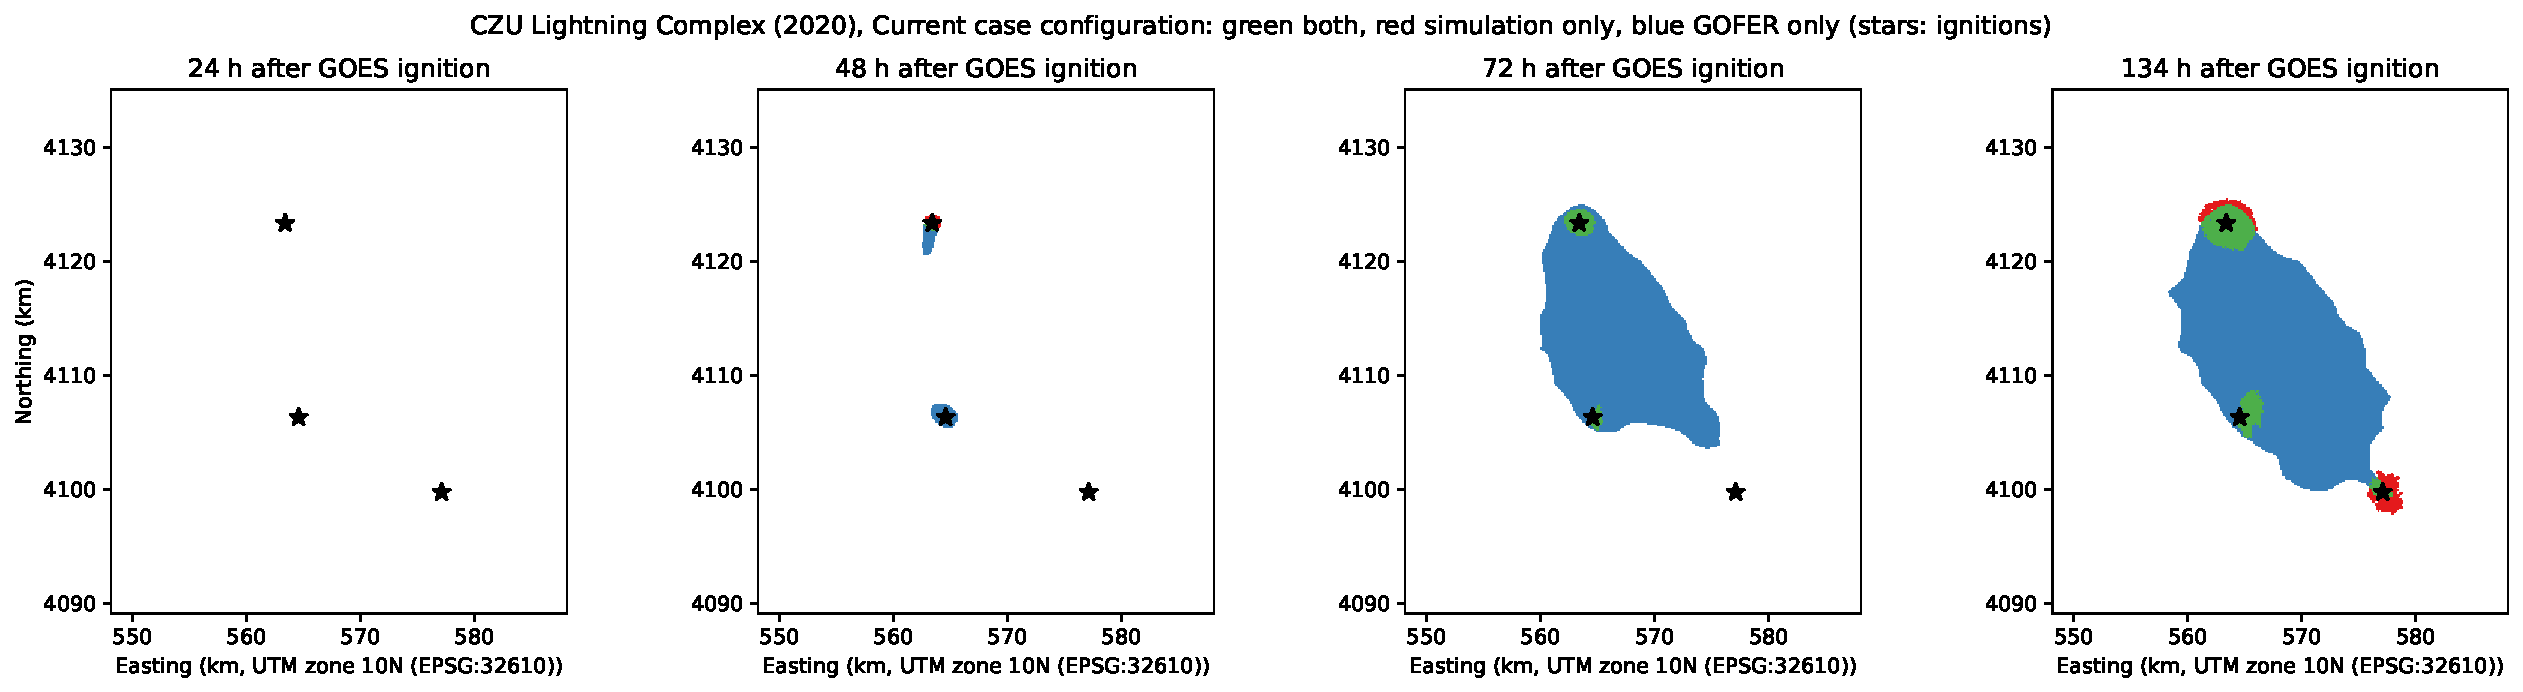
\includegraphics[width=0.98\textwidth,height=0.42\textheight,keepaspectratio]{comparison_current.pdf}
\caption{Current case configuration: simulated and GOFER-derived footprints at the fixed comparison times (hours since the GOES ignition hour) on the 30-m model grid: cells burned in both (green), only in the simulation (red), and only in the GOFER observation (blue). Stars mark the configured ignition points.}
\end{figure}

\begin{figure}[H]\centering
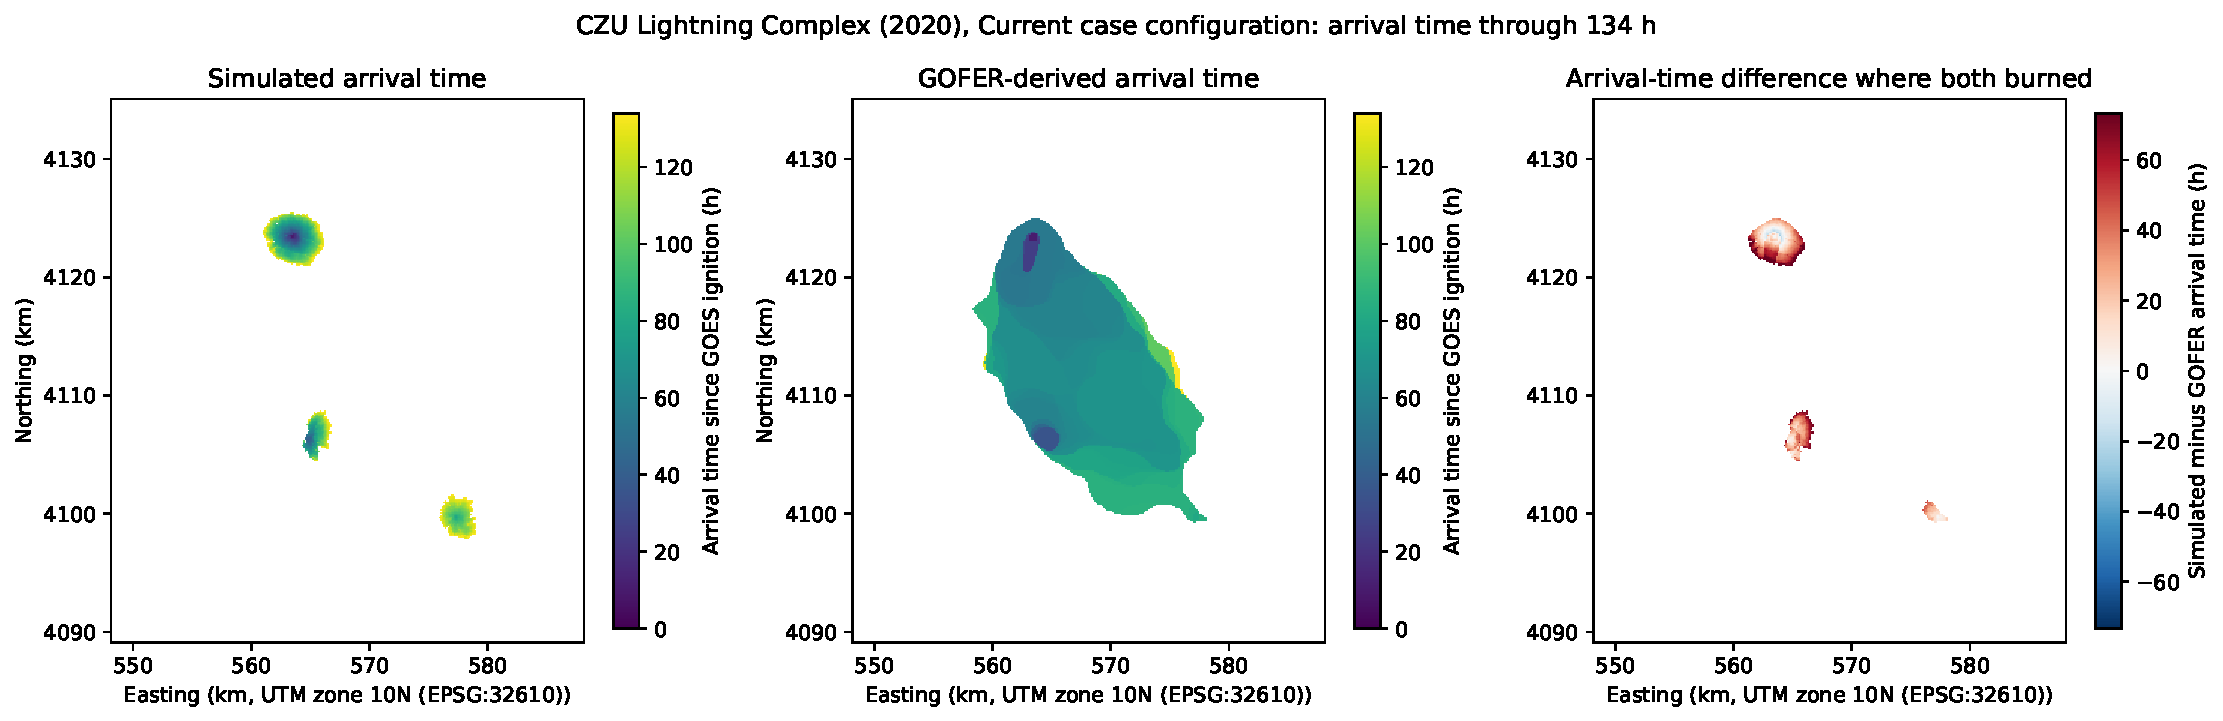
\includegraphics[width=0.98\textwidth,height=0.42\textheight,keepaspectratio]{arrival_current.pdf}
\caption{Current case configuration: simulated arrival time, GOFER-derived arrival time and their difference where both burned through the final comparison time, all in hours since the GOES ignition hour. The difference color scale is symmetric and clipped at the 95th percentile of its magnitude.}
\end{figure}

\begin{figure}[H]\centering
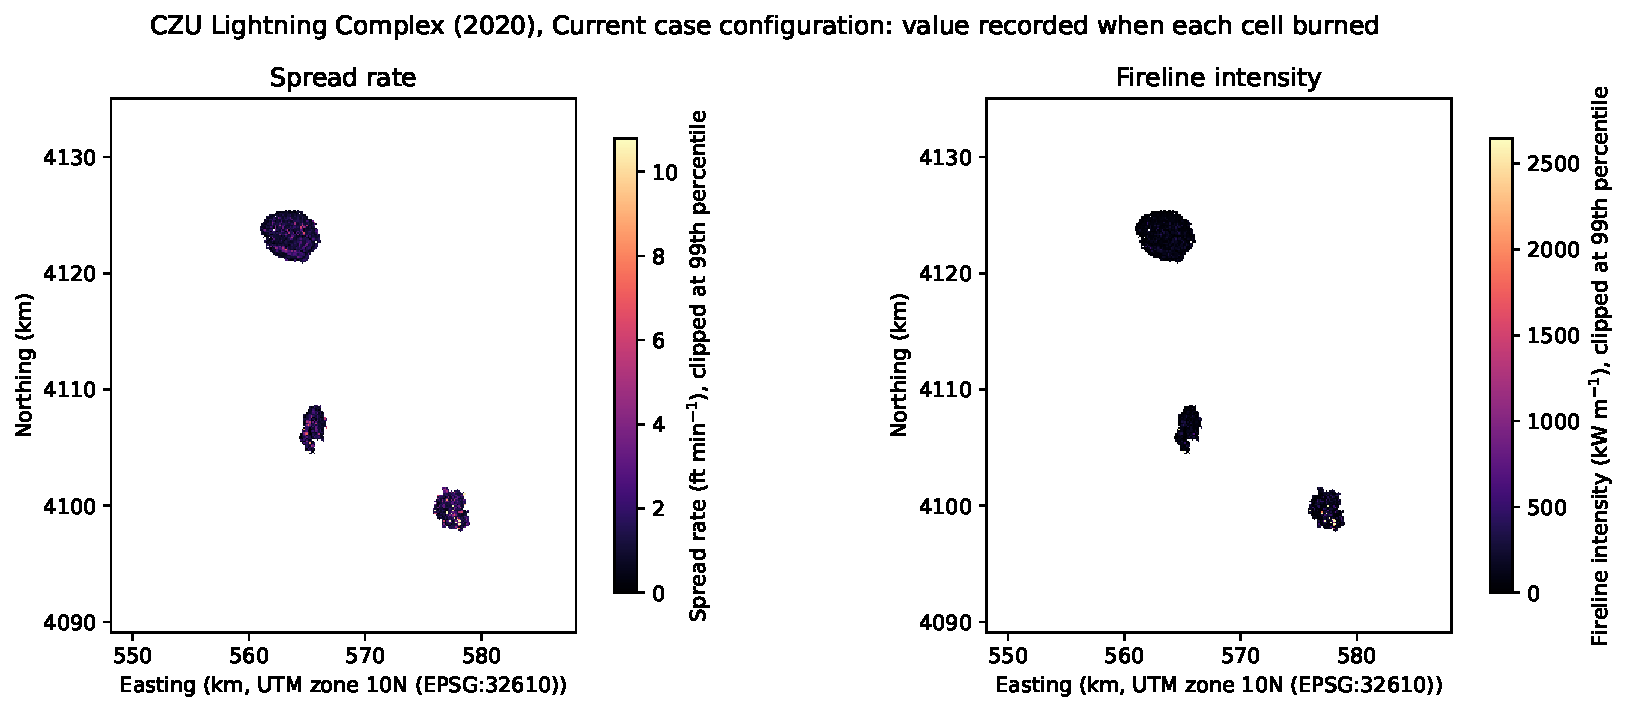
\includegraphics[width=0.98\textwidth,height=0.42\textheight,keepaspectratio]{fields_current.pdf}
\caption{Current case configuration: simulated spread rate and fireline intensity recorded when each cell burned, for the single simulation member at its final output time; color scales are clipped at the 99th percentile.}
\end{figure}

}

\newcommand{\SimulationMetrics}{%
\subsection*{Single-ignition baseline without spotting}


\textbf{NOT EVALUABLE}: No time-of-arrival result was found for this simulation.


\subsection*{Reference-case spotting configuration}


\textbf{NOT EVALUABLE}: No time-of-arrival result was found for this simulation.


\subsection*{Current case configuration}

\begin{table}[H]\centering{\small
\begin{tabular}{@{}rrrrrrrr@{}}\toprule
Time (h) & GOFER (km$^2$) & Simulated (km$^2$) & Area ratio & Jaccard & Precision & Recall & $F_1$ \\ \midrule
24 & 0.391 & 0.266 & 0.68 & 0.54 & 0.86 & 0.59 & 0.7 \\
48 & 7.38 & 2.05 & 0.277 & 0.18 & 0.69 & 0.19 & 0.3 \\
72 & 207 & 6.48 & 0.0314 & 0.031 & 1 & 0.031 & 0.061 \\
134 & 283 & 31.8 & 0.112 & 0.075 & 0.69 & 0.078 & 0.14 \\
\bottomrule\end{tabular}}
\caption{Footprint metrics of the current case configuration against the GOFER-derived footprint at fixed times since the GOES ignition hour, evaluated on the 30-m model grid over valid landscape cells. Time is the comparison instant; areas are burned areas through that instant.}
\end{table}\ReportBodyText

\begin{table}[H]\centering{\small
\begin{tabular}{@{}lr@{}}\toprule
Quantity & Value \\ \midrule
Cells burned in both by 134~h & 24{,}467 \\
Mean arrival-time difference, simulated minus GOFER (h) & 32.9 \\
Median arrival-time difference (h) & 30.1 \\
Mean absolute arrival-time difference (h) & 33.8 \\
Root-mean-square arrival-time difference (h) & 40.3 \\
Simulated end since GOES ignition (h) & 134 \\
Propagation stalled before the planned end & no \\
First contact with domain boundary (h) & none \\
Final simulated area (ac) & 7{,}858 \\
Final crown-fire area (ac) & 160 \\
\bottomrule\end{tabular}}
\caption{Arrival-time and integrated statistics of the current case configuration. Arrival-time differences use cells burned in both the simulation and the GOFER observation by the final comparison time.}
\end{table}\ReportBodyText

Precision exceeds recall at the final comparison time, so the simulated footprint lies largely inside the observation but misses much of it: the simulation undergrows or follows a displaced trajectory. The simulated burned area is 0.11 times the observed area at 134~h. Where both burned, the simulated fire arrives on average 32.9~h later than the observed fire (mean absolute difference 33.8~h).

}

\newcommand{\IntegratedResults}{%
\begin{figure}[H]\centering
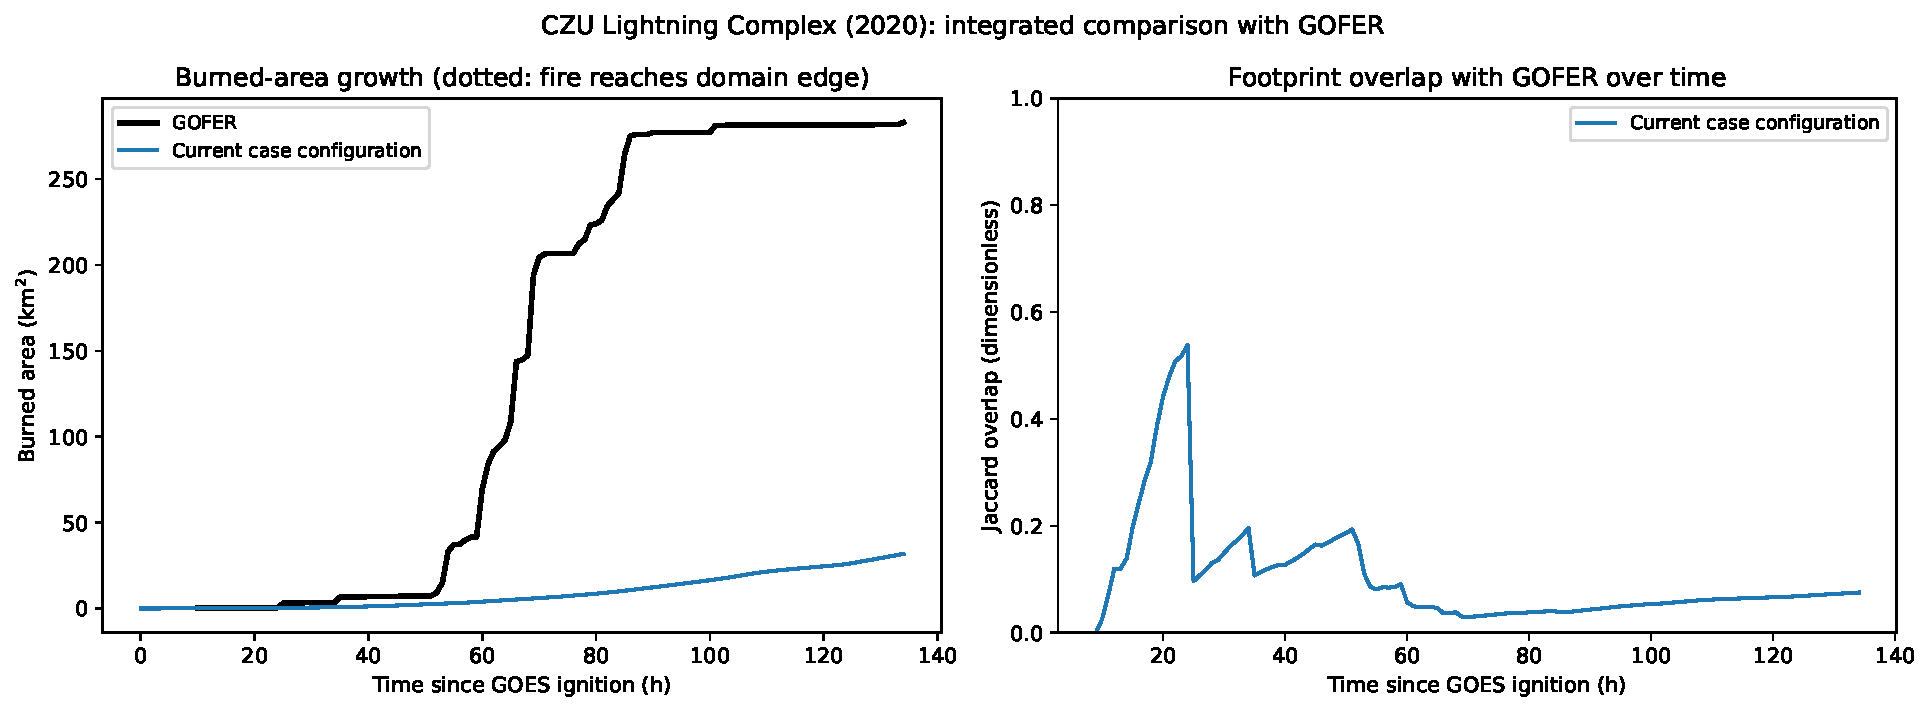
\includegraphics[width=0.98\textwidth,height=0.42\textheight,keepaspectratio]{burned_area_growth.pdf}
\caption{Observed (GOFER) and simulated burned-area growth, and the Jaccard overlap of each simulation with the GOFER footprint, evaluated hourly since the GOES ignition hour. Dotted lines mark the time each simulated fire first reaches the model-domain boundary.}
\end{figure}
}

